\section{Developing GMPE Logic Trees: A ``Good Practice'' Guide}
\label{sec:logic_tree}

(TODO) - If possible I would like some of these issues to be discussed at the meeting.

\section{Conditional Field Simulation}
\label{sec:cond_field}

The extraction of the ground motion residuals from a set of observations also opens up the possibility of implementing another type of calculation that is becoming increasingly common in seismic hazard and risk modelling, and that is conditional random field simulation. These are randomly generated fields of ground motion residuals ($z$) whose values are i) spatially correlated according to a multivariate Gaussian distribution, and ii) conditioned upon observed (known) values of the residual. This type of analysis can be critical in characterising the uncertainty in ``ShakeMaps'' (i.e. field of ground motion generated from an observed event), which in turn can provide insights into the distribution of expected or, if applied \emph{a posteriori}, observed losses (citeParketal, Crowleyetal2008, Staffordetal2012).

It has been well-established from observations of densely recorded earthquakes, that ground motion residuals are spatially correlated when stations are separated by distances typically on the order of a few tens of kilometres (cite Boore2003, JayaramBaker2008). Given the assumption of lognormality in the GMPEs, it is has also been demonstrated appropriate to model the spatial correlation in ground motion residual between two or more sites using a multivariate Gaussian distribution (cite JayaramBaker2009). The coeffiecient of correlation between two sites separated by a distance $h$ ($\rho \left( h \right)$) is shown to decay exponentially with distance such that:

\begin{equation}
\rho \left( h \right) = \exp \left( {\frac{-a\left(T\right) h}{b \left(T\right)}} \right)
\end{equation}

\noindent where $a\left( T \right)$ and $b\left( T \right)$ control the shape of the decay and are dependent on the period of ground motion under consideration. One such model of spatial correlation, which we shall use in this example, is that of cite JayaramBaker2009:

\begin{equation}
\rho \left( h \right) = \exp\left( {\frac{-3h}{b \left( T \right)}} \right) \quad \text{where} \quad b \left( T \right) = \begin{cases}\begin{cases}
8.5 + 17.2 T \text{ ``Case 1'' } & T < 1\ s\\
40.7 - 15.0 T \text{ ``Case 2'' } & T < 1\ s\end{cases}&\\
\qquad 22.0 + 3.7 T \qquad\qquad\quad T \geq 1\ s&
\end{cases}
\label{eq:jayarambaker}
\end{equation}

Consider a set of correlated random variables distributed according to a multivariate Gaussian distribution with a mean of zero and a standard deviation of unity ($\mathbf{X} = \left[ {X_1, X_2, \ldots , X_N} \right]$) and with a positive definite covariance matrix given by $\mathbf{C}$. A randomly generated sample of values can be generated via:

\begin{equation}
\mathbf{X} = \mathbf{\mu} + \mathbf{LU}
\end{equation}

\noindent where $\mathbf{\mu}$ is the mean values of the field (in this case a zero-vector $\mathbf{0}$), $\mathbf{U}$ is a sample of independent normally distributed random variates and $\mathbf{L}$ is the lower matrix defined by $\mathbf{LL^T} = \mathbf{C}$, which is obtained by Cholesky factorisation of the covariance matrix. This assumes that values of $\mathbf{X}$ are unknown \emph{a priori}, as might be the case if considering spatially correlated fields of ground motion residuals for some as yet unrecorded event. The ability to generate spatially correlated fields in this manner is supported directly by OpenQuake.

When considering a recorded event it is possible to partition the ground motion field into those locations for which the GMPE residual is known ($\mathbf{X_{OBS}}$), and those for which it is unknown ($\mathbf{X_{UNK}}$). Given the locations of both the known and unknown values the covariance matrices can be formed where $\mathbf{C_{11}}$ is the covariance of the known residuals, $\mathbf{C_{22}}$ the covariance of the unknown locations and $\mathbf{C_{12}}$ and $\mathbf{C_{21}}$ the covariance matrices considering the distance between the known and unknown locations. In the case of a multivariate standard normal distribution, the distribution of residuals at both locations can be depicted as:

\begin{equation}
\begin{bmatrix}\mathbf{X_{OBS}}\\ \hline \mathbf{X_{UNK}}\end{bmatrix} \sim N_M \left( {\begin{bmatrix}\mathbf{0} \\ \hline \mathbf{0}\end{bmatrix}, \left[ {\begin{array}{c|c}\mathbf{C_{11}} & \mathbf{C_{12}} \\ \hline \mathbf{C_{21}} & \mathbf{C_{22}}\end{array}}\right]}\right)
\end{equation}

\noindent which is arranged to give the distribution of residuals at the unknown locations, conditional upon the known residuals:
\begin{equation}
\left[ {\mathbf{X_{UNK}} | \mathbf{X_{OBS}}} \right] \sim N_M \left( {\left[ {\mathbf{C_{21}C_{11}^{-1}X_{OBS}}} \right], \left[ {\mathbf{C_{22}} - \mathbf{C_{21}C_{11}^{-1}C_{12}}}\right]}\right)
\end{equation}

From this model it is then possible to simulate random fields of GMPE residuals conditioned upon observed residuals. This functionality is not directly supported in OpenQuake, as it requires a mean by which the observed residuals can be characterised using the desired GMPE. As has been shown in Chapter \ref{chap:residuals}, however, the GMPE-SMTK does exactly this. Therefore it becomes possible to use the GMPE-SMTK, in conjunction with OpenQuake, to produce multiple fields of spatially correlated ground motions that are conditional upon a set of known observations. For this purpose we include a set of tools in a module called \verb=smtk.hazard.conditional_simulation=, which we shall import as, and subsequently refer to as, \verb=csim=

\begin{python}
import smtk.hazard.conditional_simulation as csim
\end{python}

\subsection{Example of Conditional Simulation: L'Aquila}

In the following example we consider a set of 15 records taken from the L'Aquila earthquake. In the current example these records have been put into a GMPE-SMTK database on the path \verb=/data/LAquila_Database/=, following the approach described in section \ref{sec:hdf5}. The first step in this process is to load the database and calculate the ground motion residuals:

\begin{python}[frame=single]
import cPickle
from smtk.residuals.gmpe_residuals import Residuals
# Load the database 
import cPickle
db1 = cPickle.load(open("./data/LAquila_Database/metadatafile.pkl",
                        "r"))
\end{python}

In this example we shall consider only the citeAkkaretal2014 GMPE, and just two intensity measures: PGA and $Sa \left( {1.0s} \right)$:

\begin{python}[frame=single]
gmpe_list = ["AkkarEtAlRjb2014"]
imts = ["PGA", "SA(0.2)", "SA(1.0)"]
# Calculate the residuals
resid1 = Residuals(gmpe_list, imts)
resid1.get_residuals(db1)
\end{python}

We may be interested to observe the distance trend in these residuals. This is generated using the tools described in chapter \ref{chap:residuals}, and can be seen in Figure \ref{fig:laquila_resid_distance}.

\begin{figure}[htb]
  \centering
  \begin{subfigure}[b]{0.49\textwidth}
      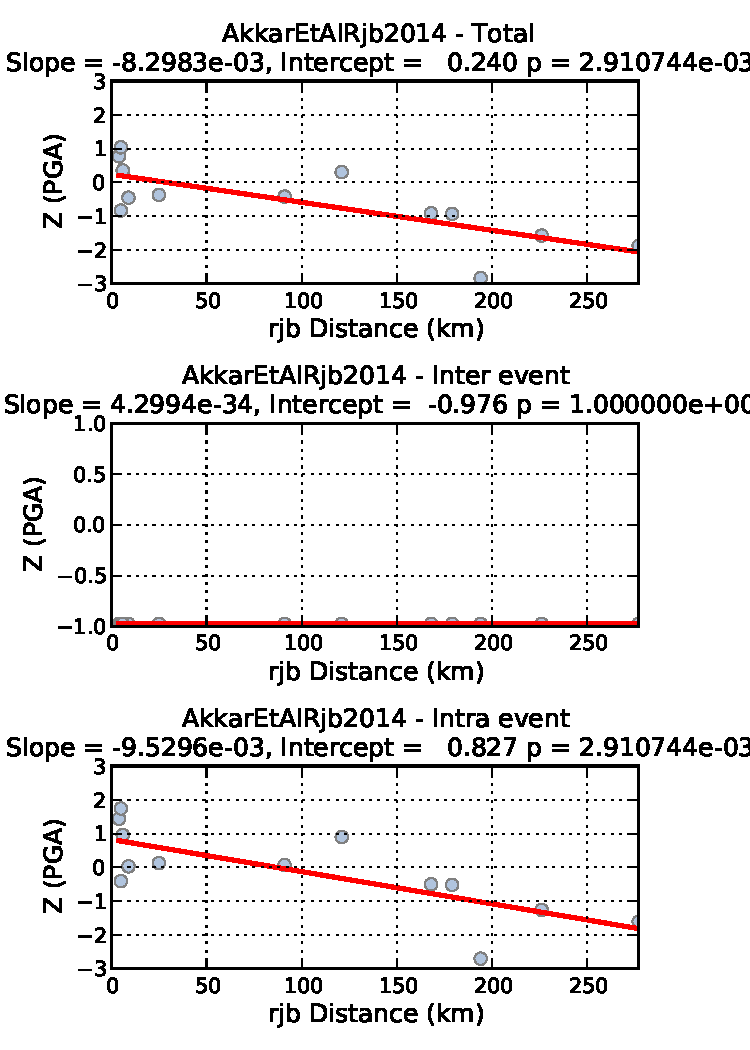
\includegraphics[width=\textwidth]{./figures/hazard/LAquila_Residuals_with_distance.pdf}
      \caption{PGA}
      \label{fig:laquila_resid_pga}
  \end{subfigure}
    \begin{subfigure}[b]{0.49\textwidth}
      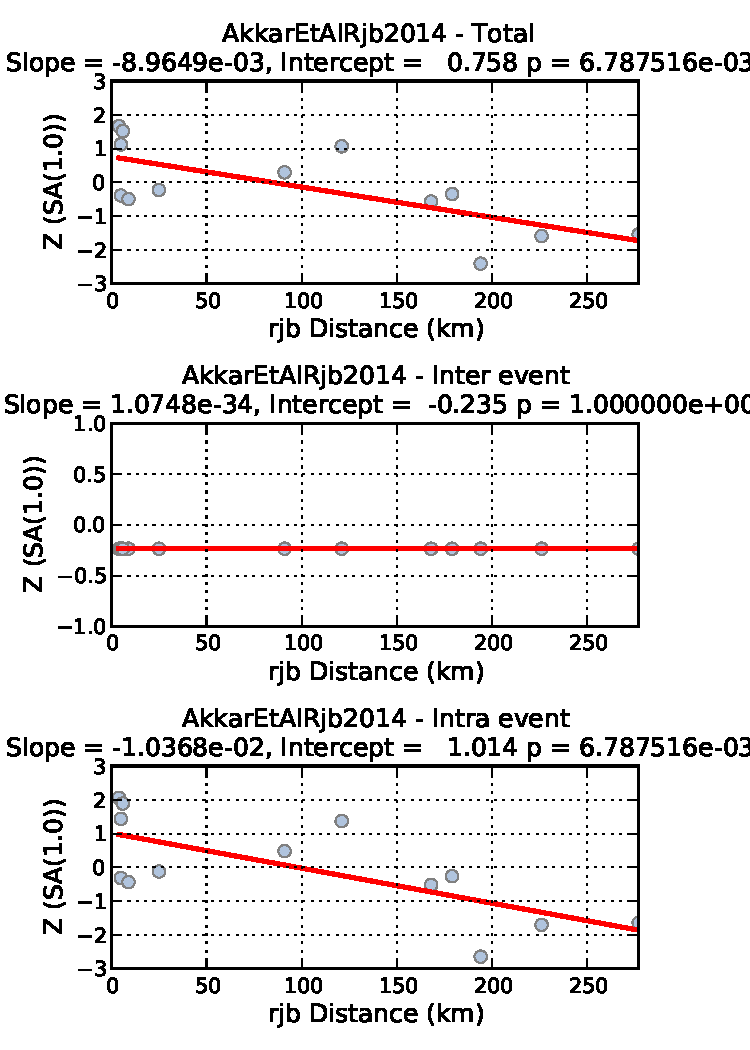
\includegraphics[width=\textwidth]{./figures/hazard/LAquila_Residuals_with_distance_sa1.pdf}
      \caption{$Sa \left( {1.0 s} \right)$ }
      \label{fig:laquila_resid_sa1}
  \end{subfigure}
  \caption{Residual trends with distance for the L'Aquila ground motion residuals}
  \label{fig:laquila_resid_distance}
\end{figure}

Here we see that for both PGA and $Sa \left( {1.0 s} \right)$ the inter-event residual is moderately negative (-0.976 for PGA and -0.235 for $Sa \left( {1.0 s} \right)$), and we observe a clear trend that the ground motions from this earthquake attenuated to a greater extent than that predicted by the GMPE. 

In the present case we have a model of the finite extent of the earthquake rupture. We put this rupture into an OpenQuake xml format\footnote{More information on the OpenQuake scenario rupture format can be found in citeCrowley2013}, as shown below, and save it in the file \verb=laquila_rupture.xml=.

\begin{verbatim}
<?xml version='1.0' encoding='utf-8'?>
<nrml xmlns:gml="http://www.opengis.net/gml"
      xmlns="http://openquake.org/xmlns/nrml/0.4">
    <simpleFaultRupture>
        <magnitude>6.3</magnitude>
        <rake>-98.0</rake>
        <hypocenter lon="13.38" lat="42.3476" depth="9.3"/>
        <simpleFaultGeometry>
                <gml:LineString>
                    <gml:posList>
                        13.3976 42.4371
                        13.5571 42.3012
                    </gml:posList>
                </gml:LineString>
            <dip>50.0</dip>
            <upperSeismoDepth>0.8</upperSeismoDepth>
            <lowerSeismoDepth>12.69</lowerSeismoDepth>
        </simpleFaultGeometry>
    </simpleFaultRupture>
</nrml>
\end{verbatim}

With the use of the OpenQuake hazardlibrary and Python's \verb=Matplotlib= plotting tools we can visualise the spatial trend in the residuals. Firstly we load in the rupture. The \verb=csim= module contains the method \verb=build_rupture_from_file=, which will load in the rupture:

\begin{python}
rupture_file = "laquila_rupture.xml"
rupture = csim.build_rupture_from_file(rupture_file)
\end{python}

For plotting it is convenient to define the outline of the surface projection of the rupture as a simple polygon:

\begin{python}
# Import the OpenQuake polygon class
from openquake.hazardlib.geo.polygon import Polygon
rupture_outline = Polygon([rupture.surface.top_left,
                           rupture.surface.top_right,
                           rupture.surface.bottom_right,
                           rupture.surface.bottom_left,
                           rupture.surface.top_left])
\end{python}

The next step is to take the database and return its locations as an instance of the class \verb=openquake.hazardlib.site.SiteCollection=. This can be done using the method within the database class (\verb=GroundMotionDatabase=) called \verb=get_site_collection=

\begin{python}
observed_sites = db1.get_site_collection()
\end{python}

The plot of the spatial distribution of residuals of PGA with respect to the rupture location is shown in Figure \ref{fig:laquila_spatial_resid}. This can be generated using the Python code below:

\begin{python}[frame=single]
# Import the Matplotlib library
import matplotlib.pyplot as plt
# Extract the PGA residuals
pga_residuals = resid1.residuals["AkkarEtAlRjb2014"]["PGA"]["Intra event"]
plt.figure(figsize=(10,8))
# Plot the rupture
plt.plot(rupture_outline.lons, rupture_outline.lats, "r-")
# Plot the reisduals
plt.scatter(observed_sites.lons, observed_sites.lats, 
            s=40,
            c=pga_residuals, 
            norm=Normalize(vmin=-3.0, vmax=3.0))
plt.title("PGA Observed Intra-event Residual", fontsize=16)
plt.colorbar()
plt.xlabel("Longitude", fontsize=14)
plt.ylabel("Latitude", fontsize=14)
\end{python}

\begin{figure}[htb]
  \centering
  \begin{subfigure}[b]{\textwidth}
      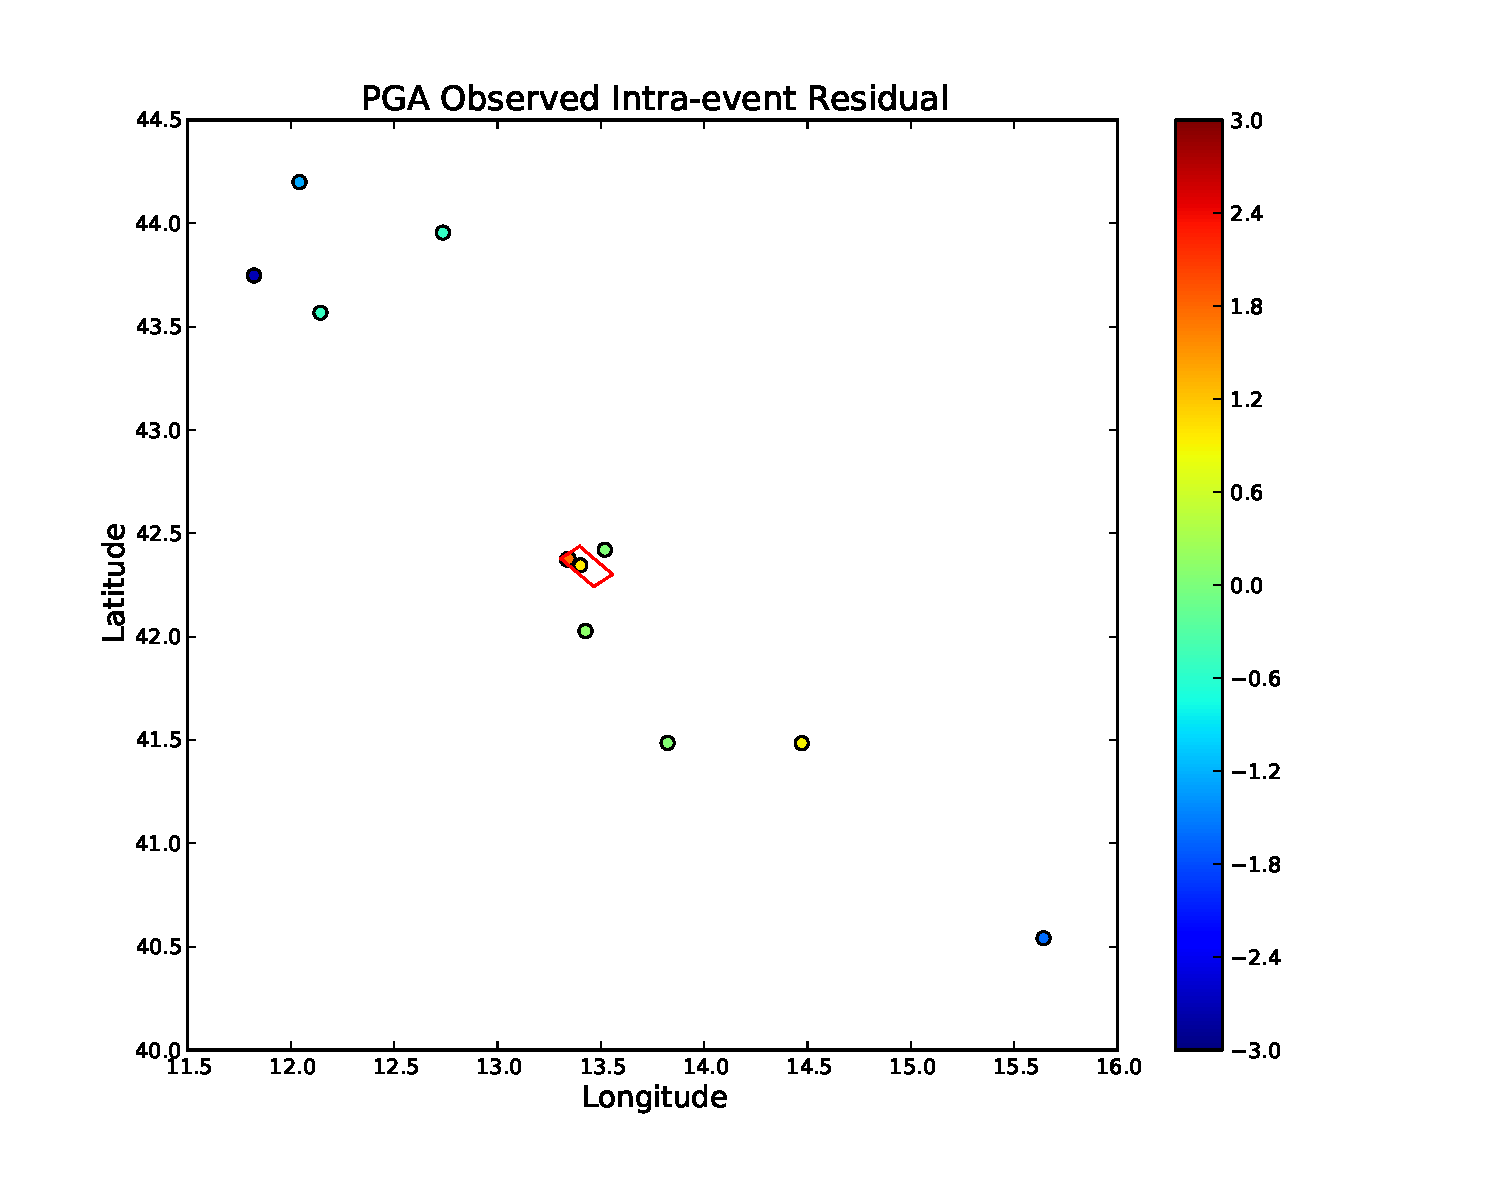
\includegraphics[trim=14mm 14mm 14mm 14mm, clip, width=0.65\textwidth]{./figures/hazard/LAquila_Observed_IntraEvent_Resid.pdf}
      \label{fig:laquila_spatial_resid_pga}
  \end{subfigure}
    \begin{subfigure}[b]{\textwidth}
      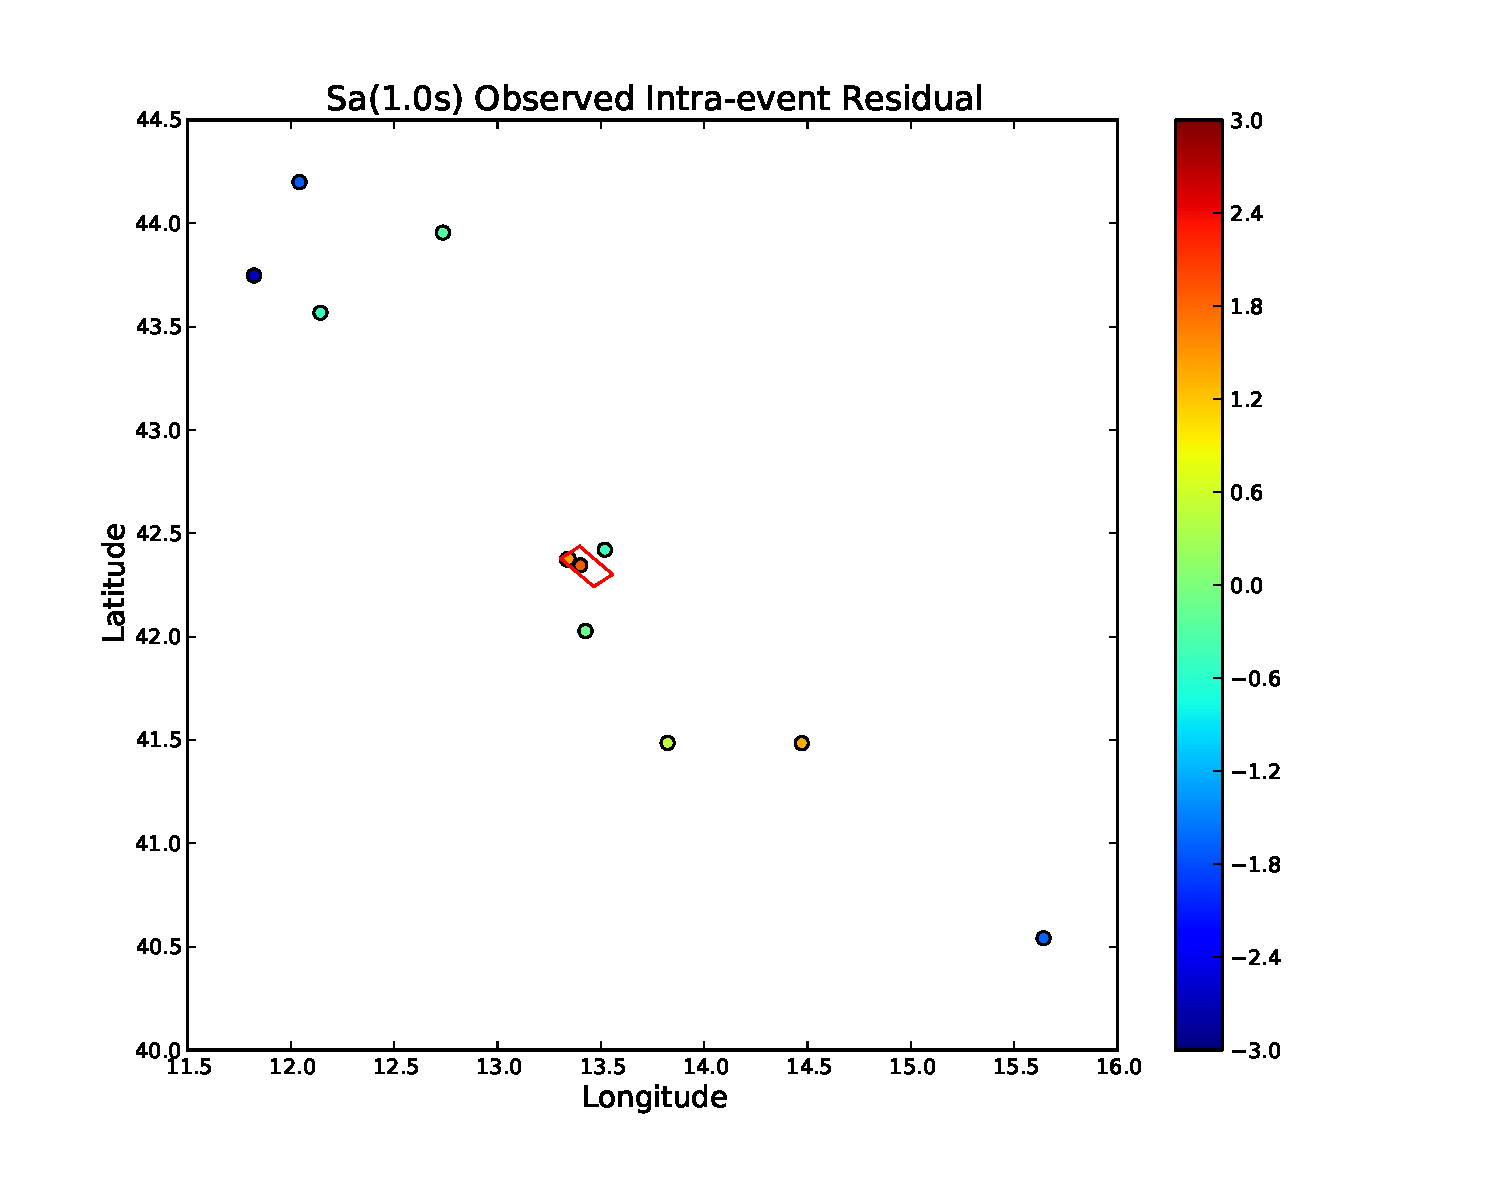
\includegraphics[trim=14mm 14mm 14mm 14mm, clip, width=0.65\textwidth]{./figures/hazard/LAquila_Observed_IntraEvent_Resid_sa1.pdf}
      \label{fig:laquila_spatial_resid_sa1}
  \end{subfigure}
  \caption{Distribution of intra-event residuals for the L'Aquila ground motion records. The surface projection of the L'Aquila rupture is shown in red.}
  \label{fig:laquila_spatial_resid}
\end{figure}

Figure \ref{fig:laquila_spatial_resid} helps understand the residual distribution further as we observed that for both intensity measures there is a small cluster of strongly positive residuals in the very near-field of the fault (due to directivity effects).

If we want to generate a spatially correlated random field of observations around the L'Aquila area, we can use the observed GMPE residuals and the spatial correlation model in equation \ref{eq:jayarambaker} to generate a realisation of a field of possible residuals. In the present example we have created a regularly spaced grid of ``target'' (i.e. unknown sites) with known soil properties. We assume this has been created as an instance of the \verb=openquake.hazardlib.site.SiteCollection= class, and we call this variable \verb=unknown_sites=. To generate a 10 random fields of spatially correlated residuals conditioned upon a set of observations we can use the \verb=csim= method \verb=conditional_simulation= as follows:

\begin{python}
# Generate fields of conditioned on the PGA residuals
output_resid_pga = csim.conditional_simulation(observed_sites,
                                               pga_residuals,
                                               unknown_sites,
                                               "PGA",
                                               nsim=10)
# Generate fields of conditioned on the Sa (1.0) residuals
output_resid_sa1 = csim.conditional_simulation(observed_sites,
                                               pga_residuals,
                                               unknown_sites,
                                               "SA(1.0)",
                                               nsim=10)
\end{python}
\noindent The output will be an array of shape $N_{SITES} \times N_{SIMULATIONS}$, where $N_{SITES}$ is the number of unknown sites and $N_{SIMULATIONS}$ the number of desired random fields (10 in this example). For a field located close to the rupture, the spatially correlated residuals are shown for both intensity meausres in Figures \ref{fig:laquila_epsilon_pga} and Figures \ref{fig:laquila_epsilon_sa1} respectively.  

\begin{figure}[htb]
	\centering
		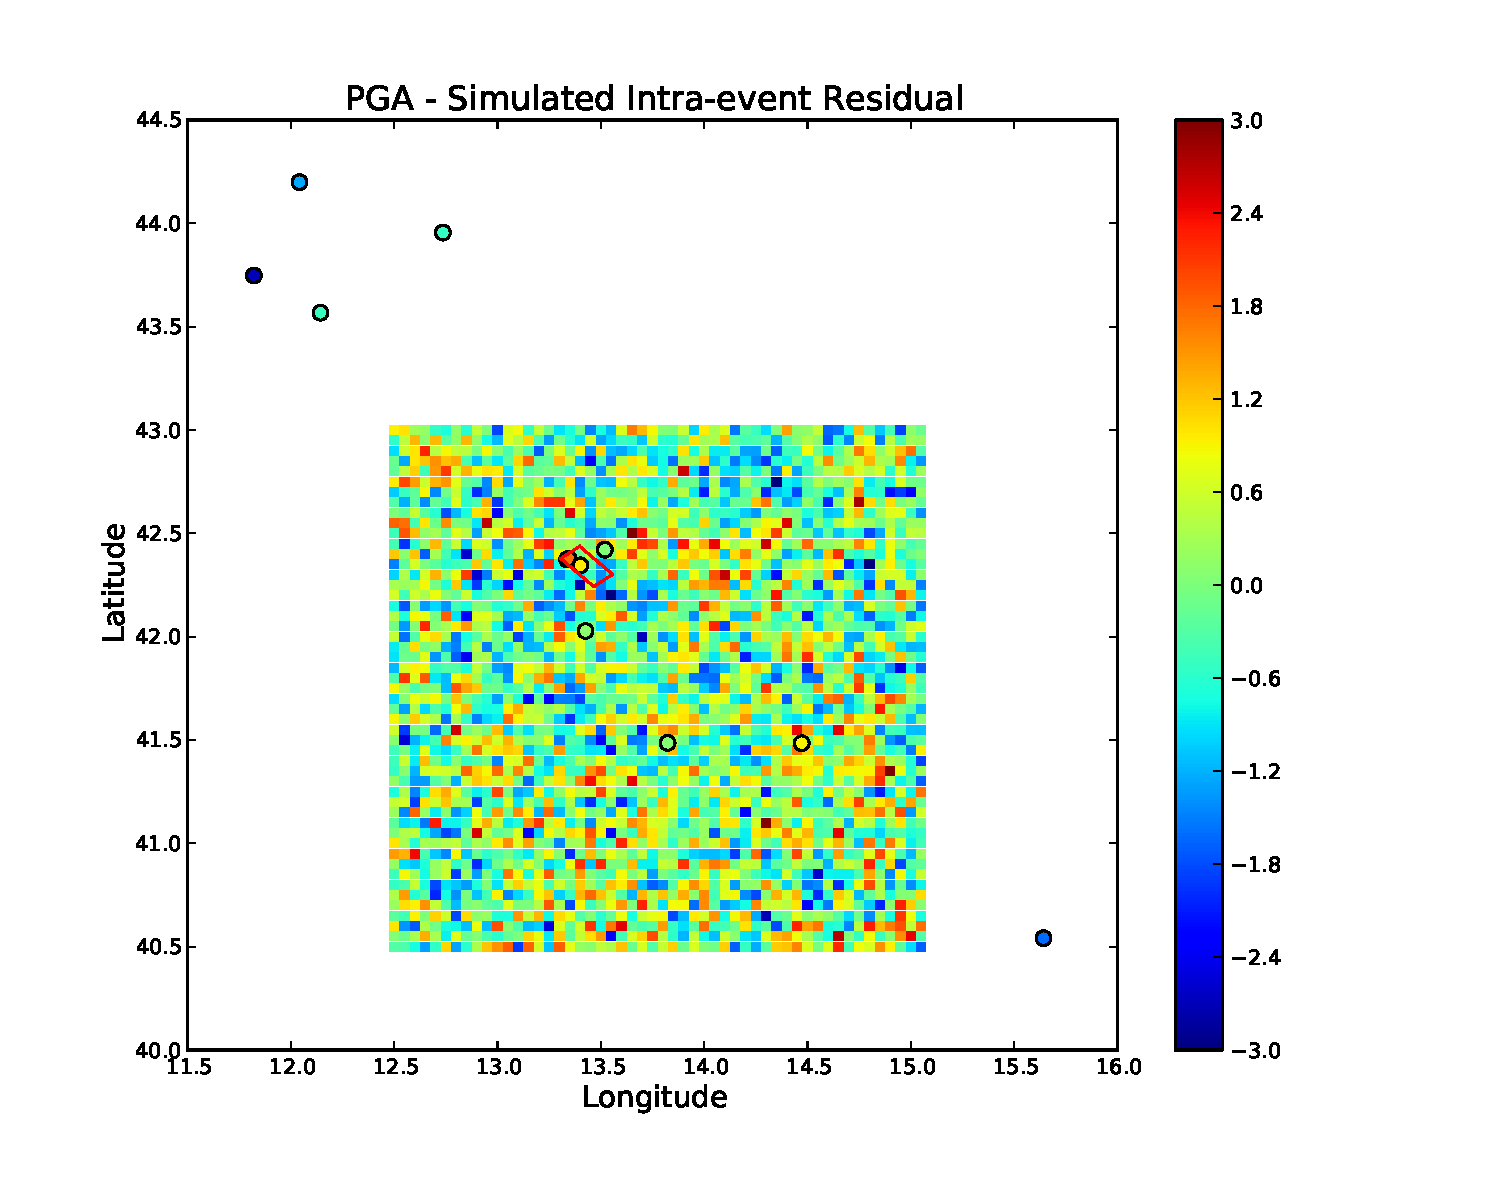
\includegraphics[trim=10mm 10mm 10mm 10mm, clip, width=0.8\textwidth]{./figures/hazard/LAquila_Simulated_Epison_PGA.pdf}
	\caption{Random field of PGA ground motion residuals conditioned upon observed residuals (circles) in the L'Aquila region}
	\label{fig:laquila_epsilon_pga}
\end{figure}
\begin{figure}[htb]
	\centering
		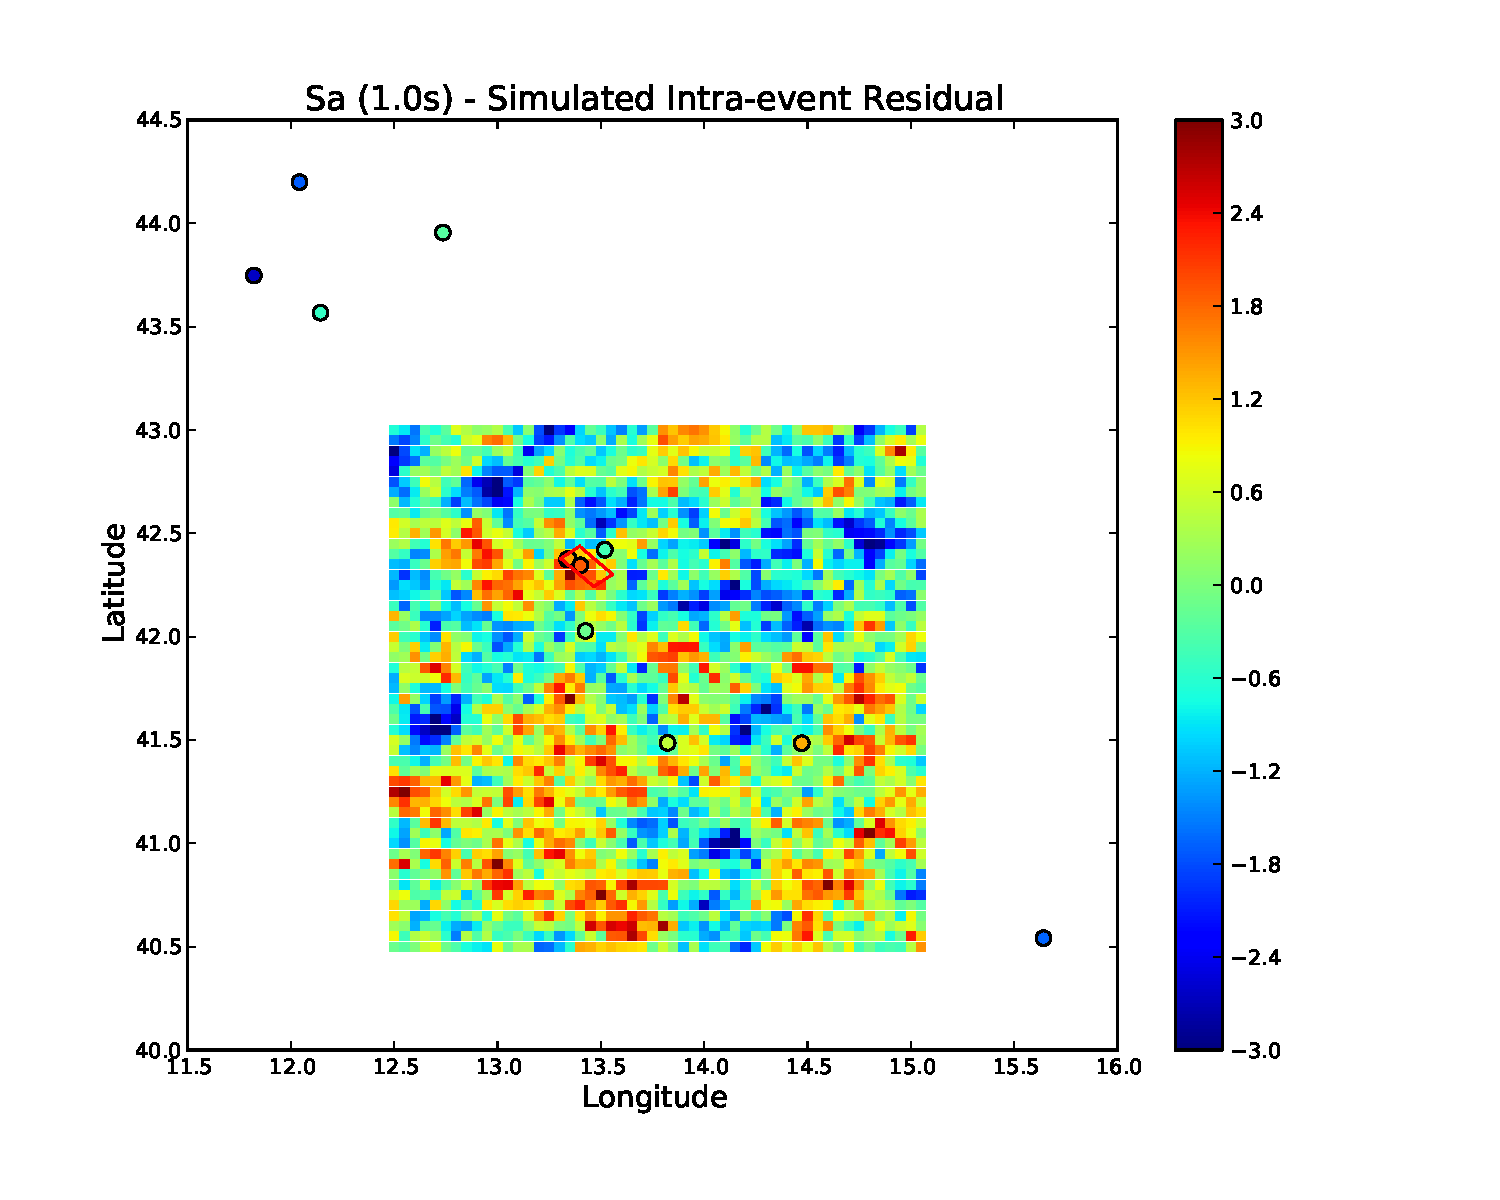
\includegraphics[trim=10mm 10mm 10mm 10mm, clip, width=0.8\textwidth]{./figures/hazard/LAquila_Simulated_Epsilon_Sa1.pdf}
	\caption{Random field of $Sa \left( {1.0 s} \right)$ ground motion residuals conditioned upon observed residuals (circles) in the L'Aquila region}
	\label{fig:laquila_epsilon_sa1}
\end{figure}

The spacing of this particular field is approximately 5 km. The typical correlation length (i.e. the distance at which $\rho \left( h \right)$ drops below 0.05) of PGA is on the order of approaximately 10 to 15 km. Given the exponential model it is evident that for PGA the spatial correlation is not so significant at this resolution. For $Sa \left( {1.0 s} \right)$ the correlation length may be on the order of 30 to 40 km; hence both the spatial correlation and the effects of the conditioning are visible clearly in Figure \ref{fig:laquila_epsilon_sa1}. Particular attention should be paid to the area of strong positive residuals in the near-field of the rupture.

The \verb=csim= tools contain a general method to implement much of the process outlined previously. This method is called \verb=get_conditional_gmfs= and its usage is illustrated below:

\begin{python}
gmfs = csim.get_conditional_gmfs(db1,
                                 rupture, 
                                 sites=unknown_sites, 
                                 gsims=["AkkarEtAlRjb2014"],
                                 imts=["PGA", "SA(1.0)"],
                                 number_simulations=5,
                                 truncation_level=3.0)
\end{python}
The above command requires as input:
\begin{enumerate}
\item The database of observed ground motions for the rupture
\item The loaded rupture model
\item The target sites as an instance of the \verb=SiteCollection= class
\item The list of GMPEs
\item The list of intensity measures
\item The number of simulations
\item The number of standard deviations at which to truncate the residuals.
\end{enumerate}

The following code snippet can be used to generate the full simulated ground motion field, similar to the examples shown in Figures \ref{fig:laquila_field_pga} and \ref{fig:laquila_field_sa1}:

\begin{python}[frame=single]
# Get one of the PGA fields from the Akkar et al GMPe
pga_field = gmfs["AkkarEtAlRjb2014"]["PGA"][:, 0]
# Setup the figure
plt.figure(figsize=(10,8))
plt.plot(rupture_outline.lons, rupture_outline.lats, "r-")
# Plot the fields
plt.scatter(unknown_sites.lons, unknown_sites.lats, 
            s=50,
            c=pga_field,
            marker="s",
            edgecolor="None",
            norm=LogNorm(vmin=0.001, vmax=1))
plt.xlim(12.5, 15.0)
plt.ylim(40.5, 43.0)
plt.title("PGA (g) - Conditional Random Field", fontsize=18)
plt.colorbar()
plt.xlabel("Longitude", fontsize=14)
plt.ylabel("Latitude", fontsize=14)
\end{python}

\begin{figure}[htb]
	\centering
		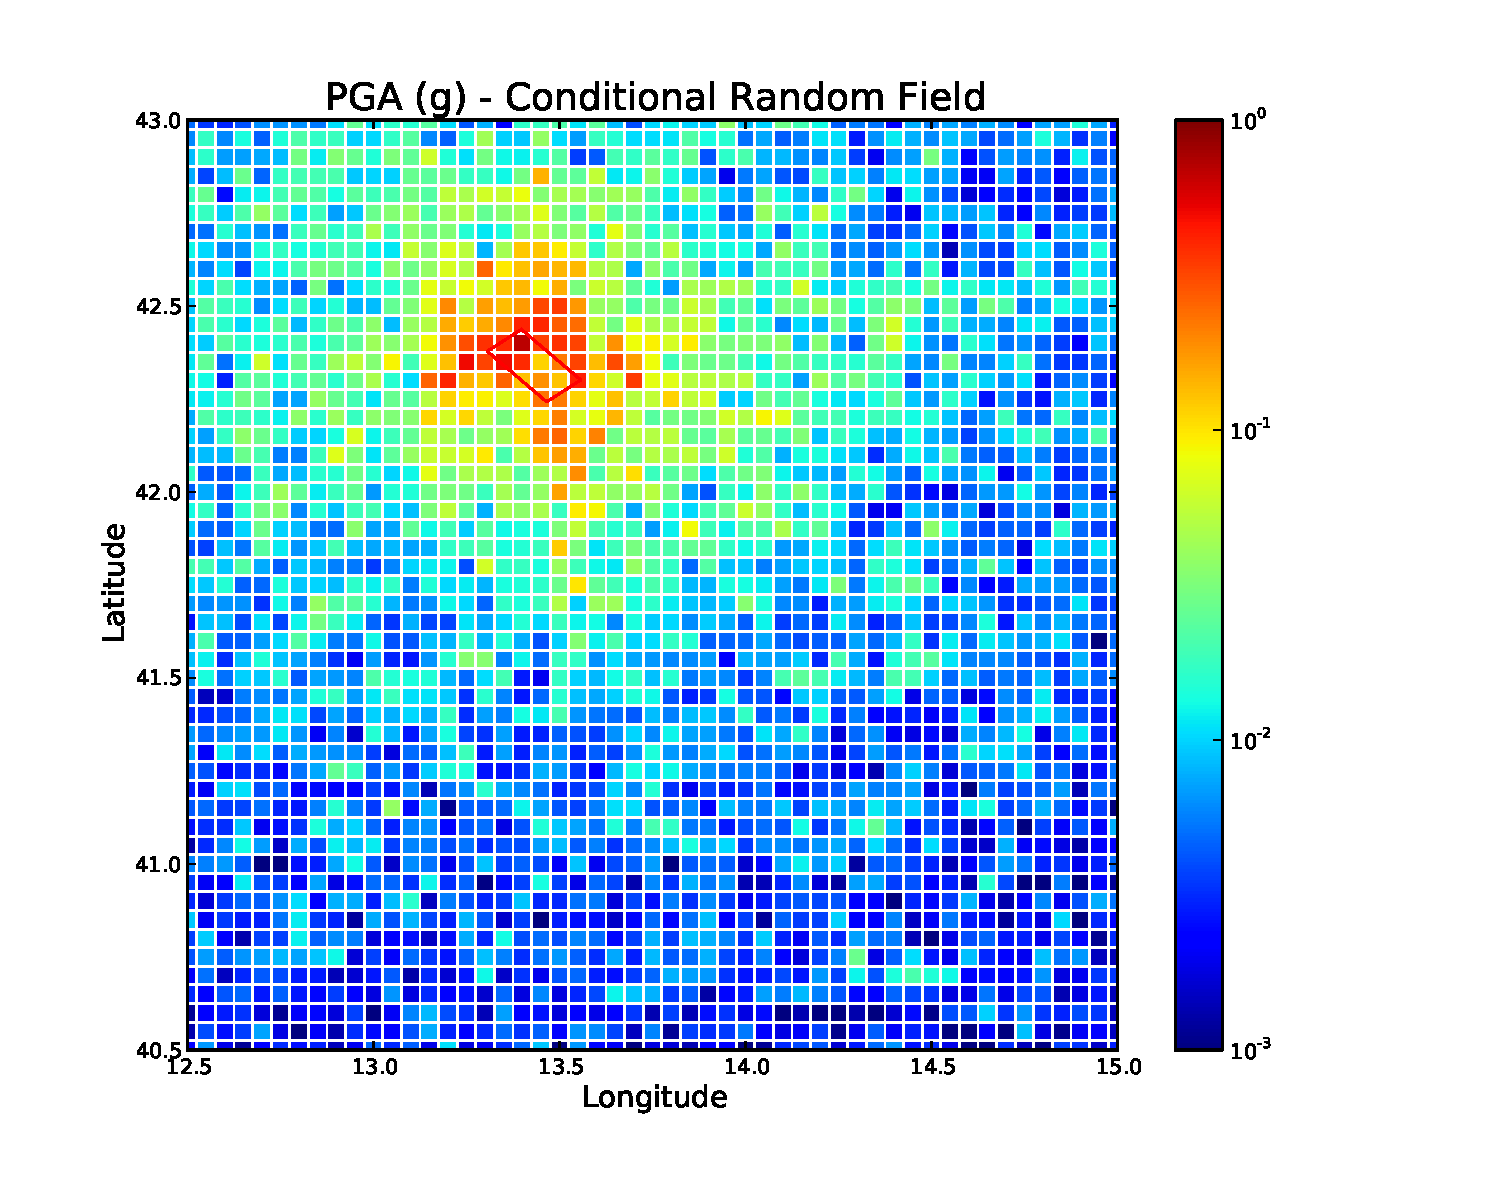
\includegraphics[trim=10mm 10mm 10mm 10mm, clip, width=0.8\textwidth]{./figures/hazard/LAquila_Conditional_Field_PGA.pdf}
	\caption{PGA ground motion field conditioned upon the ground motion residuals conditioned upon observed ground motions from the L'Aquila (2009) earthquake}
	\label{fig:laquila_field_pga}
\end{figure}
\begin{figure}[htb]
	\centering
		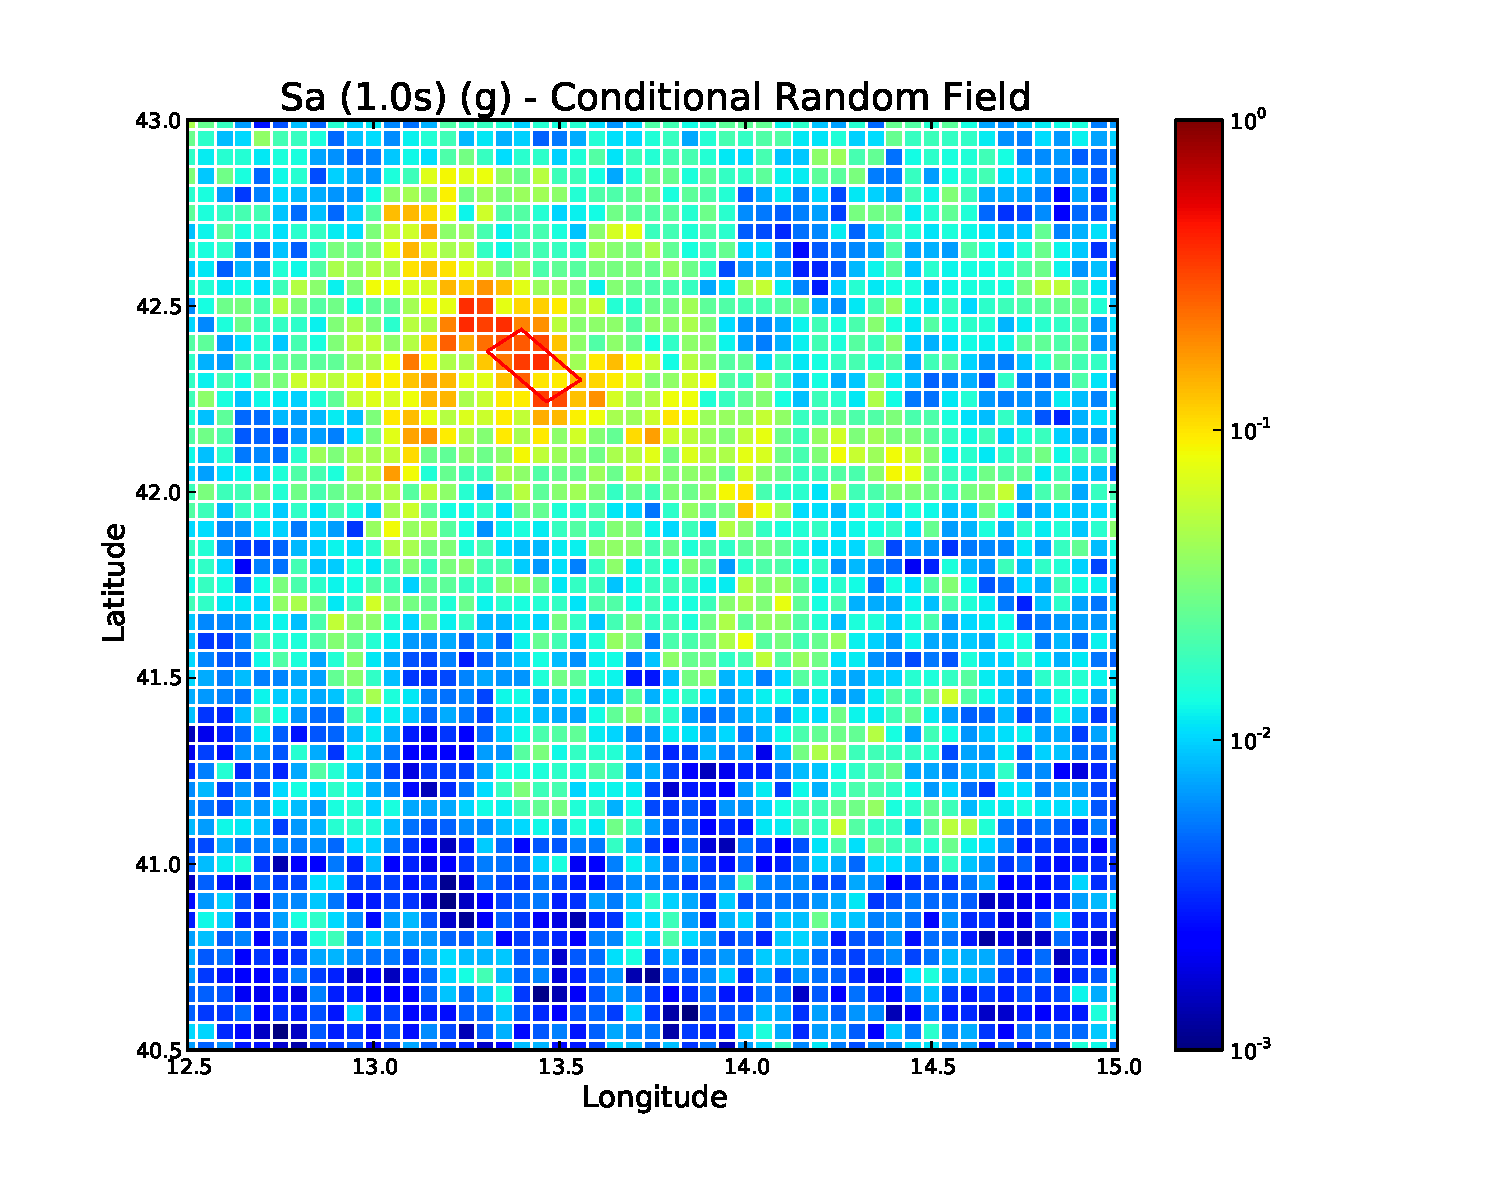
\includegraphics[trim=10mm 10mm 10mm 10mm, clip, width=0.8\textwidth]{./figures/hazard/LAquila_Conditional_Field_Sa1.pdf}
	\caption{$Sa \left( {1.0 s} \right)$ ground motion field conditioned upon the ground motion residuals conditioned upon observed ground motions from the L'Aquila (2009) earthquake}
	\label{fig:laquila_field_sa1}
\end{figure}
